\section{Durchführung}

\subsection{Aufbau}

\begin{figure}[h]
    \centering
    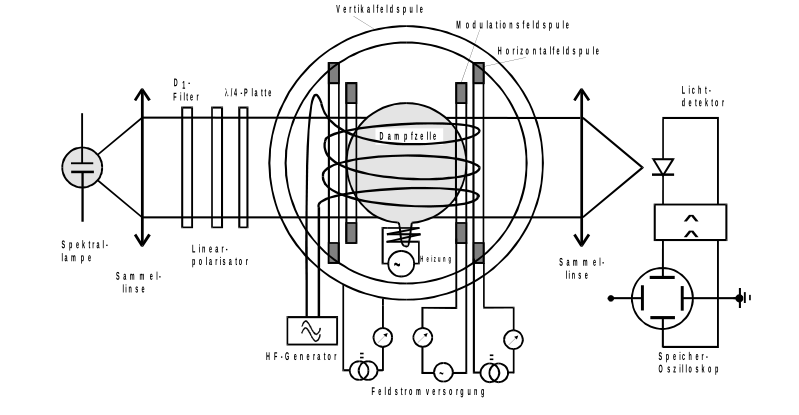
\includegraphics[width=0.7\textwidth]{latex/images/aufbau.PNG}
    \caption{Der Aufbau für das optische Pumpen schematisch dargestellt \protect \cite[V21].}
    \label{img:aufb}
\end{figure}

Der Aufbau des Versuchs ist in Abbildung \ref{img_aufb} schematisch dargestellt.\\
Er teilt sich dabei in einen optischen und einen Messaufbau auf. Der reale optische Aufbau ist in Abbildung
\ref{img:aufb_opt} zu finden und der Messaufbau in Abbildung \ref{aufb_mess }.\\
Im optischen Aufbau strahlt eine Rubidium-Spektrallampe auf eine Kollimations-Linse, die den Strahl bündelt.
Anschließend trifft das Licht auf einen Filter, der alle Frequenzen bis auf die $D_1$-Linie von Rubidium, 
mit $\lambda = \SI{794.8}{\nano\metres}$, herausfiltert. Danach wird das Licht mit einer $\frac{\lambda}{4}$-Platte zirkular polarisiert.\\
Dieses Licht trifft dann auf die Dampfzelle, welche den Rubidium-Dampf enthält. 
Der Dampf wird mit einem kleinen Ofen erwärmt, um den optimalen Dampfdruck zu erzeugen.
Dies sollte eine halbe Stunde vor den Messungen geschehen.\\
Die Dampfzelle ist von drei Helmholtzspulen und einer weiteren Spule umgeben.


\subsection{Durchführung}